\documentclass[12pt,a4paper]{article}
\usepackage[UTF8]{ctex}
\usepackage{graphicx}
\usepackage{hyperref}
\usepackage{geometry}
\usepackage{enumitem}
\usepackage{float}

\geometry{a4paper,left=2.5cm,right=2.5cm,top=2.5cm,bottom=2.5cm}

\title{实验报告3:识别运行进程}
\author{学生姓名}
\date{\today}

\begin{document}

\maketitle
\tableofcontents
\newpage

\section{实验目标}

本实验将使用Windows Sysinternals Suite中的TCP/UDP Endpoint Viewer工具来识别计算机上运行的进程。具体目标如下:

\begin{itemize}
    \item 下载Windows Sysinternals Suite
    \item 启动TCP/UDP Endpoint Viewer
    \item 探索运行中的进程
    \item 探索用户启动的进程
\end{itemize}

\section{实验背景}

在本实验中,我们将探索进程。进程是正在执行的程序或应用程序。我们将使用Windows Sysinternals Suite中的Process Explorer来探索进程,并且还将启动和观察一个新进程。

\section{实验步骤}

\subsection{第一部分:下载Windows Sysinternals Suite}

\begin{enumerate}
    \item 导航到以下链接下载Windows Sysinternals Suite:\\
    \url{https://technet.microsoft.com/en-us/sysinternals/bb842062.aspx}
    \item 下载完成后,右键单击zip文件,选择"全部提取...",从文件夹中提取文件。
    \item 选择默认名称和目标位置(Downloads文件夹),然后单击"提取"。
    \item 退出Web浏览器。
\end{enumerate}

\subsection{第二部分:启动TCP/UDP Endpoint Viewer}

\begin{enumerate}
    \item 导航到包含所有提取文件的SysinternalsSuite文件夹。
    \item 打开Tcpview.exe。当提示时,接受Process Explorer许可协议。
    \item 单击"是"允许此应用对设备进行更改。
    \item 退出文件资源管理器并关闭所有当前运行的应用程序。
\end{enumerate}

\begin{figure}[H]
    \centering
    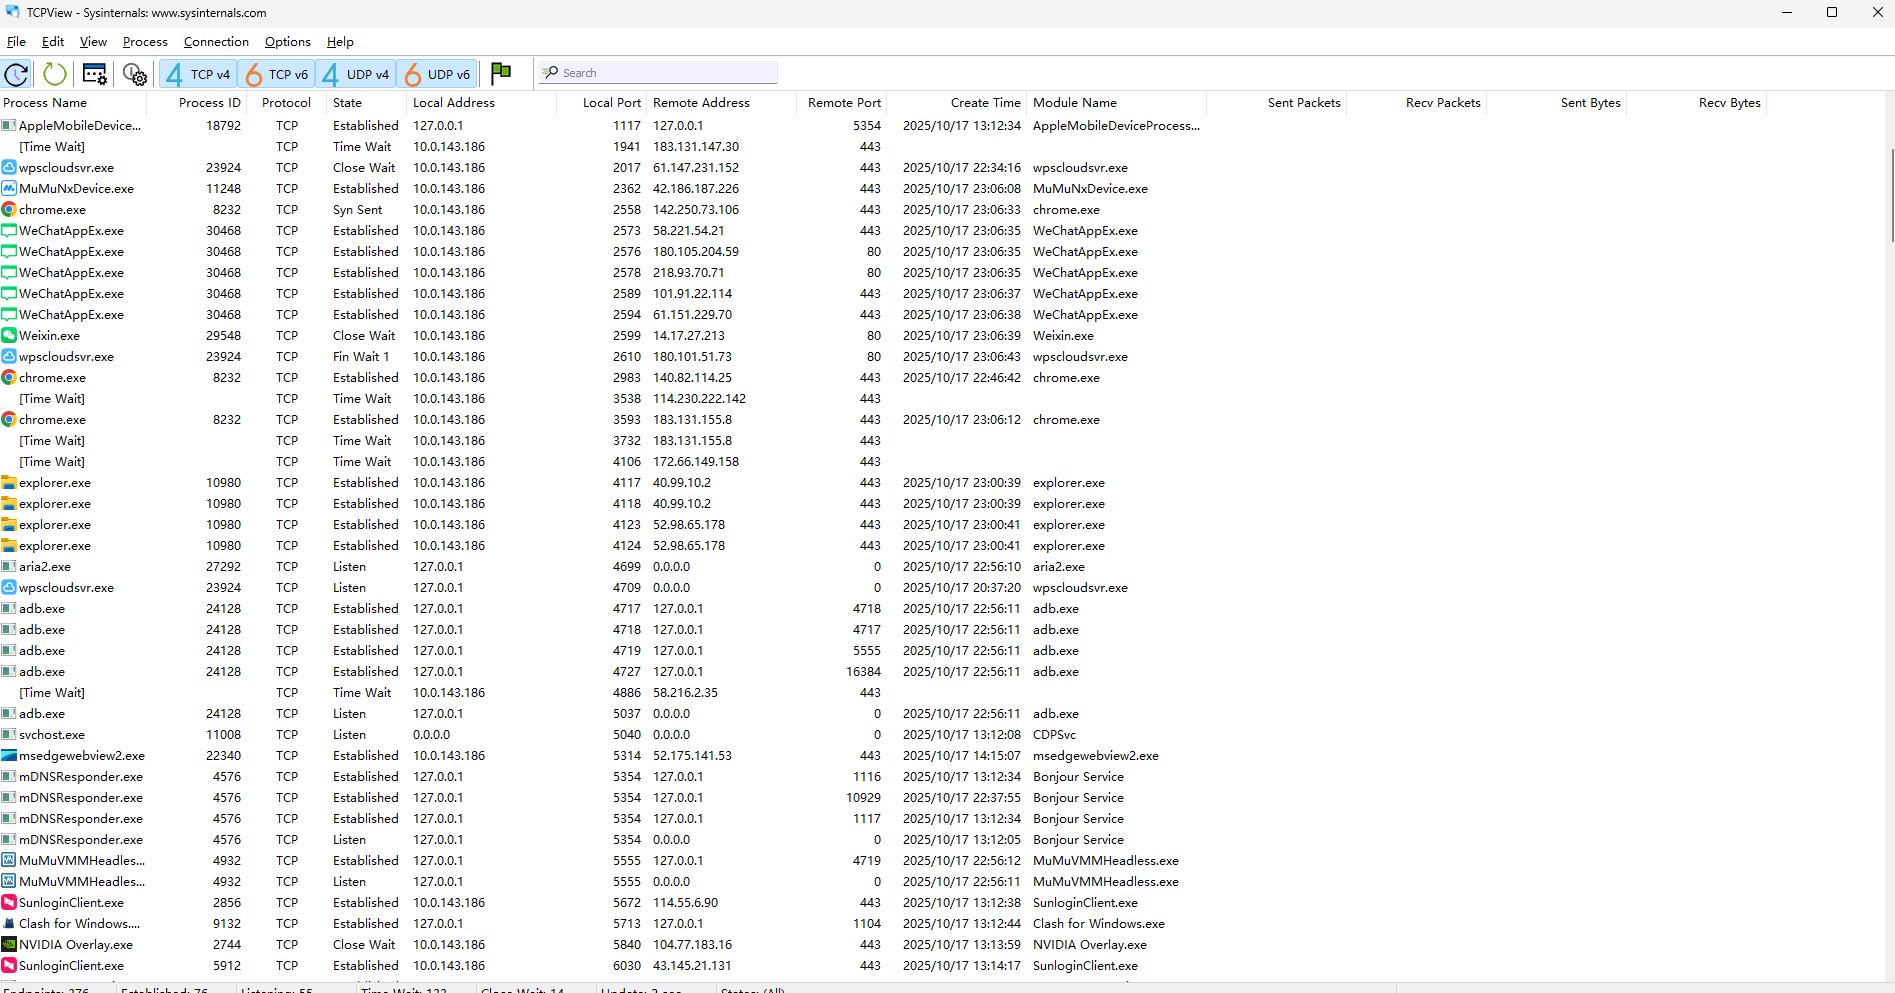
\includegraphics[width=0.8\textwidth]{TcpView.png}
    \caption{TCP/UDP Endpoint Viewer界面}
    \label{fig:tcpview}
\end{figure}

\subsection{第三部分:探索运行中的进程}

\begin{enumerate}
    \item TCPView列出了Windows PC上当前运行的进程。此时,只有Windows进程在运行。
    \item 双击lsass.exe。
\end{enumerate}

\begin{figure}[H]
    \centering
    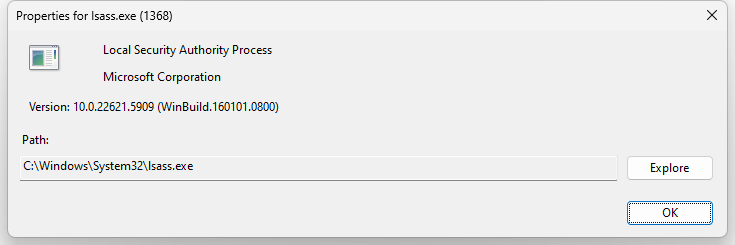
\includegraphics[width=0.8\textwidth]{lssas.png}
    \caption{lsass.exe进程属性}
    \label{fig:lsass}
\end{figure}

\textbf{问题:}
\begin{itemize}
    \item lsass.exe是什么?它位于哪个文件夹中?
\end{itemize}

\textbf{回答:}
lsass.exe是Windows本地安全认证子系统服务(Local Security Authority Subsystem Service)的可执行文件。它负责执行安全策略、验证用户登录Windows系统、管理密码更改以及创建访问令牌。从图中可以看出,它位于C:/Windows/System32文件夹中。这是一个关键的Windows系统进程,如果被终止,系统将变得不稳定或强制重启。

\begin{enumerate}
    \item[3.] 完成后关闭lsass.exe的属性窗口。
    \item[4.] 查看其他运行进程的属性。
\end{enumerate}

\textbf{注意:}并非所有进程都可以查询属性信息。

\subsection{第四部分:探索用户启动的进程}

\begin{enumerate}
    \item 打开Web浏览器,如Microsoft Edge。
\end{enumerate}

\begin{figure}[H]
    \centering
    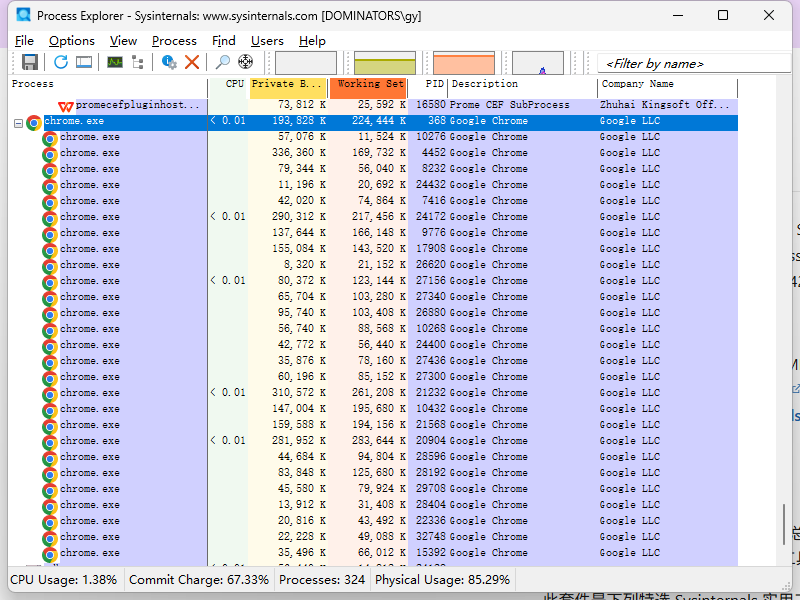
\includegraphics[width=0.8\textwidth]{proecxp.png}
    \caption{Process Explorer检测浏览器进程}
    \label{fig:procexp}
\end{figure}

\textbf{问题:}
\begin{itemize}
    \item 您在TCPView窗口中观察到了什么?
\end{itemize}

\textbf{回答:}
在TCPView窗口中,当打开Web浏览器(如Microsoft Edge)时,可以观察到多个新的网络连接被创建。这些连接显示了浏览器进程与各种远程服务器之间建立的TCP/UDP连接。可以看到浏览器进程使用了不同的本地端口与远程服务器通信,包括DNS查询(用于域名解析)、HTTP/HTTPS连接(用于加载网页内容)以及其他可能的连接(如WebSocket、内容分发网络等)。这些连接的状态(如ESTABLISHED、LISTENING、CLOSE\_WAIT等)也会显示在TCPView中。

\begin{enumerate}
    \item[2.] 关闭Web浏览器。
\end{enumerate}

\textbf{问题:}
\begin{itemize}
    \item 您在TCPView窗口中观察到了什么?
\end{itemize}

\textbf{回答:}
当关闭Web浏览器后,在TCPView窗口中可以观察到与浏览器相关的所有连接都消失了。这表明当应用程序被关闭时,其相关的网络连接也会被终止。TCPView会通过颜色变化(通常是红色)短暂显示这些被关闭的连接,然后它们会从列表中完全消失。系统返回到只显示基本的Windows系统进程的网络连接状态。

\section{实验二:探索进程、线程、句柄和Windows注册表}

\subsection{第一部分:探索进程}

\begin{figure}[H]
    \centering
    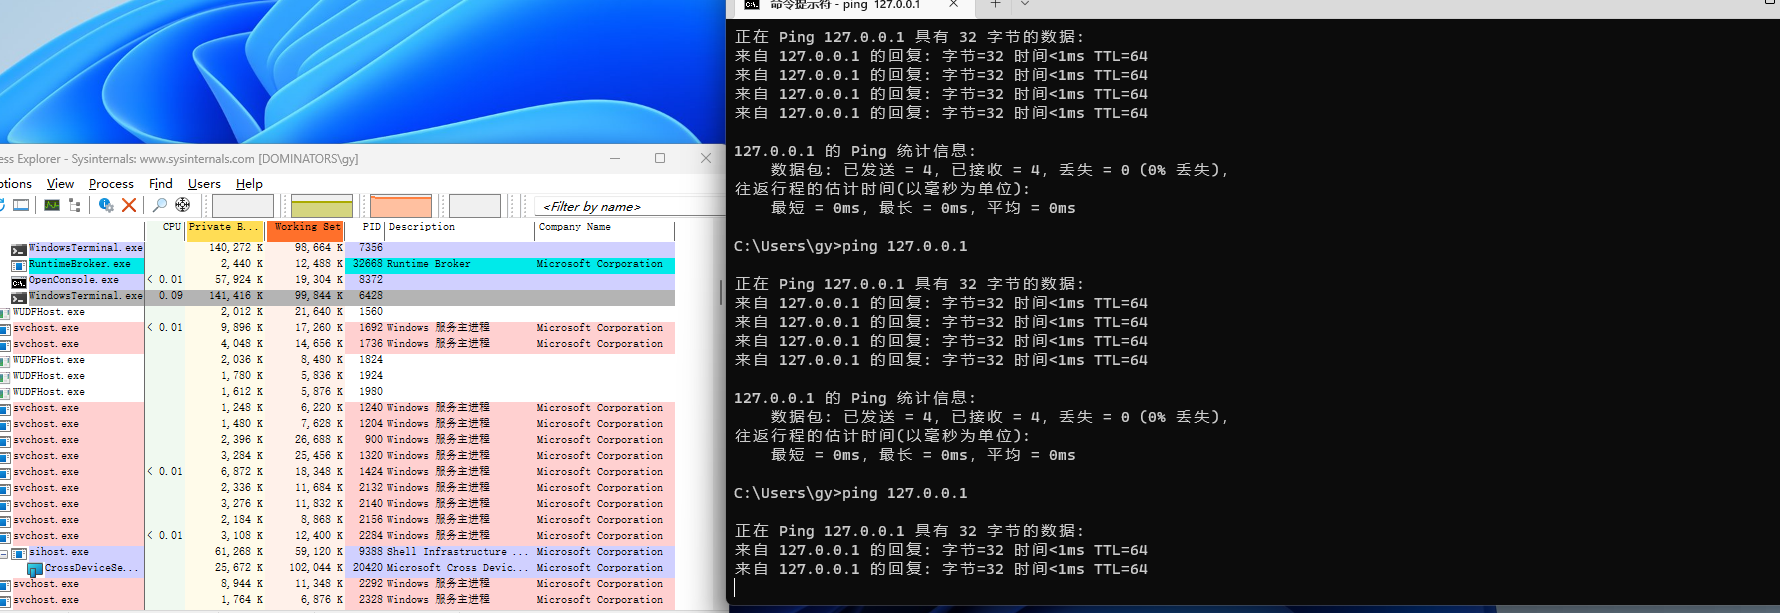
\includegraphics[width=0.8\textwidth]{cmd.png}
    \caption{Process Explorer检测命令提示符进程}
    \label{fig:cmd}
\end{figure}

\textbf{问题:}
\begin{itemize}
    \item 当进程被终止时,Web浏览器窗口发生了什么?
\end{itemize}

\textbf{回答:}
当使用Process Explorer终止Web浏览器进程时,浏览器窗口立即关闭,没有任何警告或保存提示。这是因为终止进程会强制结束该进程的所有线程和资源,不给应用程序任何机会执行正常的关闭程序(如保存数据或关闭连接)。这可能导致未保存的数据丢失,并且可能在某些情况下导致浏览历史记录或会话数据的丢失。

\textbf{问题:}
\begin{itemize}
    \item 在ping过程中发生了什么?
\end{itemize}

\textbf{回答:}
在执行ping命令期间,可以在Process Explorer中观察到cmd.exe进程下出现了新的活动。具体来说,可以看到CPU使用率有小幅波动,表明ping命令正在执行网络操作。在线程视图中,可以看到负责执行ping命令的线程处于活动状态。此外,还可以观察到与网络相关的句柄被创建和使用,这些句柄用于发送ICMP请求包和接收响应包。ping命令本身不会创建新的子进程,而是在cmd.exe进程内部作为一个命令执行。

\textbf{问题:}
\begin{itemize}
    \item 当cmd.exe进程被终止时,子进程conhost.exe发生了什么?
\end{itemize}

\textbf{回答:}
当cmd.exe进程被终止时,其子进程conhost.exe(控制台主机进程)也会被自动终止。这是因为conhost.exe是为cmd.exe提供控制台窗口服务的进程,它们之间存在父子关系。在Windows中,当父进程被终止时,操作系统通常会终止所有相关的子进程。这种行为确保了不会有孤立的进程继续运行,从而防止资源泄漏和系统不稳定。

\subsection{第二部分:探索线程和句柄}

\begin{figure}[H]
    \centering
    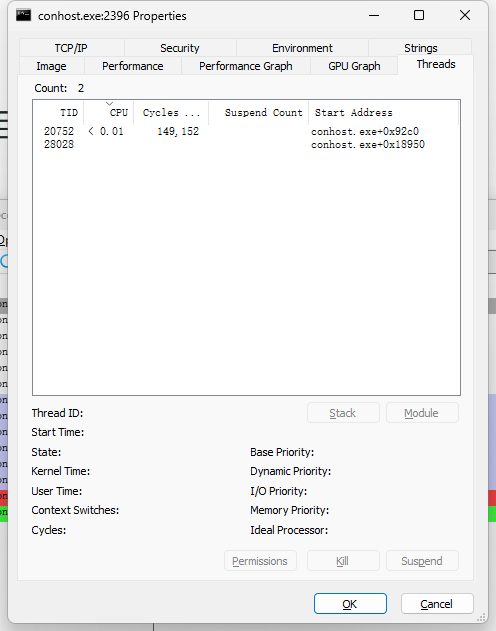
\includegraphics[width=0.8\textwidth]{Thread.png}
    \caption{进程线程属性}
    \label{fig:thread}
\end{figure}

\textbf{问题:}
\begin{itemize}
    \item 在线程属性窗口中有什么类型的信息可用?
\end{itemize}

\textbf{回答:}
在线程属性窗口中,可以看到以下类型的信息:
\begin{itemize}
    \item 线程ID(TID):每个线程的唯一标识符
    \item 线程的CPU使用率和执行时间
    \item 线程的优先级和状态(如运行中、等待、挂起等)
    \item 线程的启动地址和当前执行位置
    \item 线程栈信息,显示函数调用层次
    \item 线程上下文切换次数
    \item 线程所属的模块(DLL)
    \item 线程的创建时间
\end{itemize}
这些信息对于理解进程内部的执行流程和诊断性能问题非常有用。

\begin{figure}[H]
    \centering
    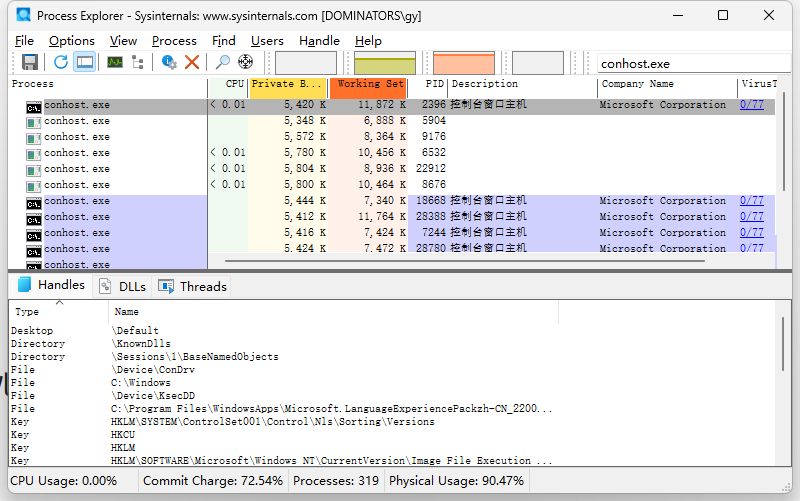
\includegraphics[width=0.8\textwidth]{handles.png}
    \caption{进程句柄属性}
    \label{fig:handles}
\end{figure}

\textbf{问题:}
\begin{itemize}
    \item 句柄指向什么?
\end{itemize}

\textbf{回答:}
在Process Explorer的句柄视图中,可以看到句柄指向各种系统资源,包括:
\begin{itemize}
    \item 文件:进程打开的文件,包括可执行文件、配置文件、数据文件等
    \item 注册表键:进程访问的Windows注册表项
    \item 目录:进程访问的文件系统目录
    \item 事件(Event):用于进程间同步的事件对象
    \item 互斥体(Mutex):用于控制对共享资源访问的同步对象
    \item 信号量(Semaphore):用于控制资源访问计数的同步对象
    \item 线程:进程创建或访问的线程对象
    \item 进程:当前进程引用的其他进程
    \item 设备:硬件设备或虚拟设备的引用
    \item 端口:通信端口,如命名管道或网络端口
\end{itemize}
这些句柄本质上是操作系统资源的引用,进程通过这些句柄与系统资源交互。

\subsection{第三部分:探索Windows注册表}

\begin{figure}[H]
    \centering
    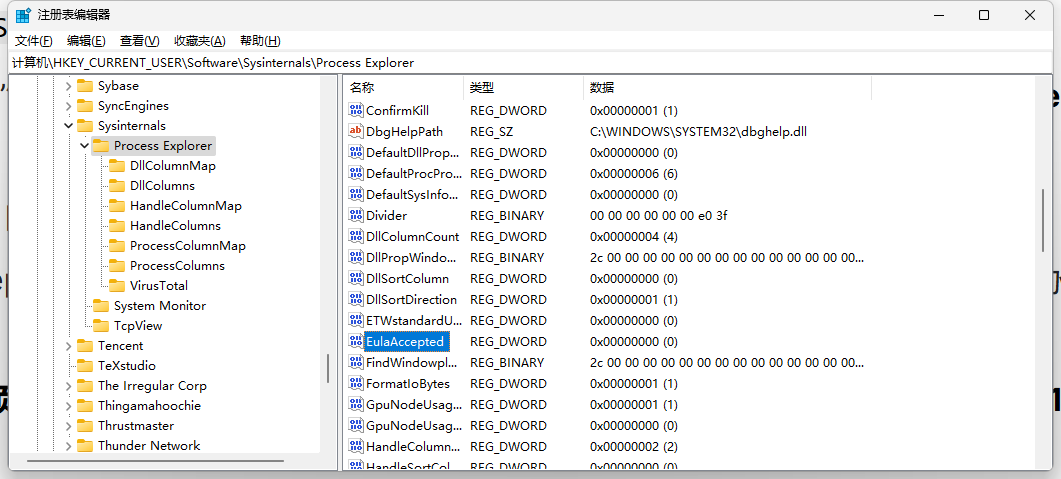
\includegraphics[width=0.8\textwidth]{Eula.png}
    \caption{注册表中的EULA设置}
    \label{fig:eula}
\end{figure}

\textbf{问题:}
\begin{itemize}
    \item EulaAccepted注册表键的值是什么?
\end{itemize}

\textbf{回答:}
EulaAccepted注册表键的值是0x00000001(1),表示用户已经接受了Process Explorer的最终用户许可协议(EULA)。这个值存储在HKEY\_CURRENT\_USER\\Software\\Sysinternals\\Process Explorer路径下。当值为1时,表示EULA已被接受;当值为0时,表示EULA尚未被接受。

\begin{figure}[H]
    \centering
    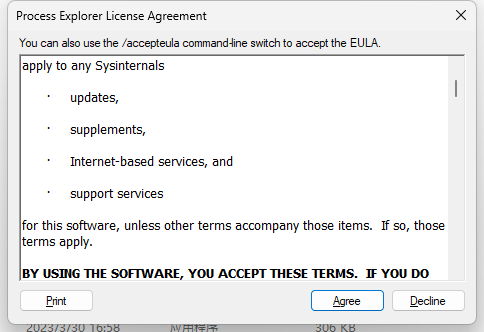
\includegraphics[width=0.8\textwidth]{Eula_0_result.png}
    \caption{将EulaAccepted值改为0后的结果}
    \label{fig:eula_result}
\end{figure}

\textbf{问题:}
\begin{itemize}
    \item 当您将EulaAccepted值从1改为0后打开Process Explorer时看到了什么?
\end{itemize}

\textbf{回答:}
当将EulaAccepted值从1改为0后打开Process Explorer时,软件会再次显示最终用户许可协议(EULA)对话框,要求用户重新接受许可条款。这表明Process Explorer在每次启动时都会检查注册表中的这个值,以确定是否需要显示EULA。如果用户接受EULA,该值会被重新设置为1;如果用户拒绝接受,应用程序将不会启动。这是软件确保用户了解并同意使用条款的一种机制。

\section{实验结论}

通过本实验,我们成功使用了Windows Sysinternals Suite中的工具来探索和分析Windows系统中的进程、线程、句柄和注册表。我们了解了:

\begin{itemize}
    \item 如何使用TCP/UDP Endpoint Viewer和Process Explorer监控系统进程
    \item 进程的层次结构和父子关系
    \item 线程作为进程内的执行单元的特性和属性
    \item 句柄如何作为进程与系统资源交互的引用
    \item Windows注册表如何存储应用程序配置信息
    \item 如何通过修改注册表值来改变应用程序行为
\end{itemize}

这些知识对于系统管理、安全分析和软件开发都非常重要,能够帮助我们更好地理解Windows操作系统的内部工作机制。

\end{document}